\documentclass[../../main.tex]{subfiles}


\begin{document}

\subsection*{(a)}
After selecting the three specified attributes, normalization by Z-transformation is done. The result is multiplied so it can be fed to all k-means clusterers at once. For each clustering we set the necessary 'k' and 'max runs' and select the 'add as label' checkbox so the cluster labels are added as a new column. To use the unscaled dataset we first reverse the Z-transformation by De-Normalizing and then apply it to the clustered data.\\  
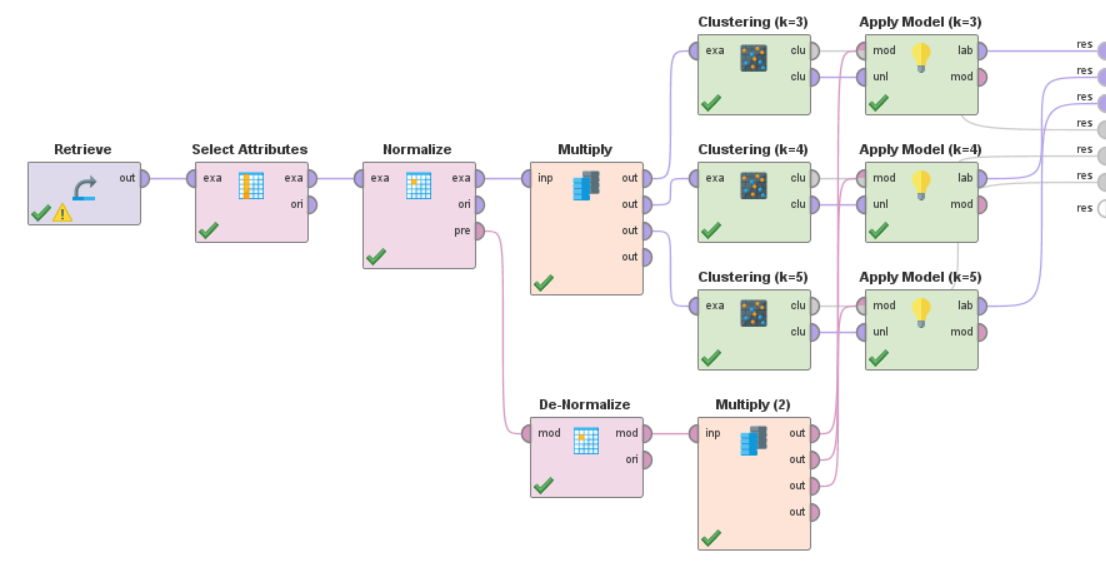
\includegraphics[width=\textwidth]{img/QUESTION_3a_PROCESS.png}



\subsection*{(b)}


\end{document}